\documentclass[class=article, crop=false]{standalone}
\usepackage[subpreambles=true]{standalone}
\usepackage{import}
\usepackage{ebproof}
\usepackage[utf8]{inputenc}
\usepackage{tikz}
\usepackage{hyperref}
\usepackage{amsmath}
\usepackage{amssymb}
\usepackage{listings}
\usepackage{verbatim}
\usepackage{a4wide}

\usepackage{subcaption}

\ifstandalone
\lstdefinelanguage{efflang}
{
    % list of keywords
    morekeywords={
        let,
        perform,
        continue,
        val,
        effect,
        in,
        if, then, else,
        with, handle, handler,
        finally,
        match
    },
    sensitive=false,
    morecomment=[s]{(*}{*)},
    morestring=[b]"
}

% Define Colors
\usepackage{color}
\definecolor{eclipseBlue}{RGB}{42,0.0,255}
\definecolor{eclipseGreen}{RGB}{63,127,95}
\definecolor{eclipsePurple}{RGB}{127,0,85}
\definecolor{bg}{RGB}{248,248,248}

\lstset{
    language={efflang},
    basicstyle=\small\ttfamily, % Global Code Style
    captionpos=b, % Position of the Caption (t for top, b for bottom)
    extendedchars=true, % Allows 256 instead of 128 ASCII characters
    tabsize=2, % number of spaces indented when discovering a tab 
    columns=fixed, % make all characters equal width
    keepspaces=true, % does not ignore spaces to fit width, convert tabs to spaces
    showstringspaces=false, % lets spaces in strings appear as real spaces
    breaklines=true, % wrap lines if they don't fit
    %frame=trbl, % draw a frame at the top, right, left and bottom of the listing
    %frameround=tttt, % make the frame round at all four corners
    framesep=4pt, % quarter circle size of the round corners
    numbers=left, % show line numbers at the left
    numberstyle=\tiny\ttfamily, % style of the line numbers
    commentstyle=\color{eclipseGreen}, % style of comments
    keywordstyle=\color{eclipsePurple}, % style of keywords
    stringstyle=\color{eclipseBlue}, % style of strings
    xleftmargin=.05\textwidth,
    framexleftmargin=17pt,
    backgroundcolor=\color{bg}
    %xrightmargin=.2\textwidth
}
\else
\lstdefinelanguage{efflang}
{
    % list of keywords
    morekeywords={
        let,
        perform,
        continue,
        val,
        effect,
        in,
        if, then, else,
        with, handle, handler,
        finally,
        match
    },
    sensitive=false,
    morecomment=[s]{(*}{*)},
    morestring=[b]"
}

% Define Colors
\usepackage{color}
\definecolor{eclipseBlue}{RGB}{42,0.0,255}
\definecolor{eclipseGreen}{RGB}{63,127,95}
\definecolor{eclipsePurple}{RGB}{127,0,85}
\definecolor{bg}{RGB}{248,248,248}

\lstset{
    language={efflang},
    basicstyle=\small\ttfamily, % Global Code Style
    captionpos=b, % Position of the Caption (t for top, b for bottom)
    extendedchars=true, % Allows 256 instead of 128 ASCII characters
    tabsize=2, % number of spaces indented when discovering a tab 
    columns=fixed, % make all characters equal width
    keepspaces=true, % does not ignore spaces to fit width, convert tabs to spaces
    showstringspaces=false, % lets spaces in strings appear as real spaces
    breaklines=true, % wrap lines if they don't fit
    %frame=trbl, % draw a frame at the top, right, left and bottom of the listing
    %frameround=tttt, % make the frame round at all four corners
    framesep=4pt, % quarter circle size of the round corners
    numbers=left, % show line numbers at the left
    numberstyle=\tiny\ttfamily, % style of the line numbers
    commentstyle=\color{eclipseGreen}, % style of comments
    keywordstyle=\color{eclipsePurple}, % style of keywords
    stringstyle=\color{eclipseBlue}, % style of strings
    xleftmargin=.05\textwidth,
    framexleftmargin=17pt,
    backgroundcolor=\color{bg}
    %xrightmargin=.2\textwidth
}
\fi

\ifstandalone
\lstdefinelanguage{scheme}
{
    % list of keywords
    morekeywords={
        define
    },
    sensitive=false,
    morecomment=[s]{\#|}{|\#},
    morestring=[b]"
}

% Define Colors
\usepackage{color}
\definecolor{eclipseBlue}{RGB}{42,0.0,255}
\definecolor{eclipseGreen}{RGB}{63,127,95}
\definecolor{eclipsePurple}{RGB}{127,0,85}

\lstset{
    language={scheme},
    basicstyle=\small\ttfamily, % Global Code Style
    captionpos=b, % Position of the Caption (t for top, b for bottom)
    extendedchars=true, % Allows 256 instead of 128 ASCII characters
    tabsize=2, % number of spaces indented when discovering a tab 
    columns=fixed, % make all characters equal width
    keepspaces=true, % does not ignore spaces to fit width, convert tabs to spaces
    showstringspaces=false, % lets spaces in strings appear as real spaces
    breaklines=true, % wrap lines if they don't fit
    frame=trbl, % draw a frame at the top, right, left and bottom of the listing
    frameround=tttt, % make the frame round at all four corners
    framesep=4pt, % quarter circle size of the round corners
    numbers=left, % show line numbers at the left
    numberstyle=\tiny\ttfamily, % style of the line numbers
    commentstyle=\color{eclipseGreen}, % style of comments
    keywordstyle=\color{eclipsePurple}, % style of keywords
    stringstyle=\color{eclipseBlue}, % style of strings
    xleftmargin=.13\textwidth,
    xrightmargin=.13\textwidth
}
\else
\lstdefinelanguage{scheme}
{
    % list of keywords
    morekeywords={
        define
    },
    sensitive=false,
    morecomment=[s]{\#|}{|\#},
    morestring=[b]"
}

% Define Colors
\usepackage{color}
\definecolor{eclipseBlue}{RGB}{42,0.0,255}
\definecolor{eclipseGreen}{RGB}{63,127,95}
\definecolor{eclipsePurple}{RGB}{127,0,85}

\lstset{
    language={scheme},
    basicstyle=\small\ttfamily, % Global Code Style
    captionpos=b, % Position of the Caption (t for top, b for bottom)
    extendedchars=true, % Allows 256 instead of 128 ASCII characters
    tabsize=2, % number of spaces indented when discovering a tab 
    columns=fixed, % make all characters equal width
    keepspaces=true, % does not ignore spaces to fit width, convert tabs to spaces
    showstringspaces=false, % lets spaces in strings appear as real spaces
    breaklines=true, % wrap lines if they don't fit
    frame=trbl, % draw a frame at the top, right, left and bottom of the listing
    frameround=tttt, % make the frame round at all four corners
    framesep=4pt, % quarter circle size of the round corners
    numbers=left, % show line numbers at the left
    numberstyle=\tiny\ttfamily, % style of the line numbers
    commentstyle=\color{eclipseGreen}, % style of comments
    keywordstyle=\color{eclipsePurple}, % style of keywords
    stringstyle=\color{eclipseBlue}, % style of strings
    xleftmargin=.13\textwidth,
    xrightmargin=.13\textwidth
}
\fi

\renewcommand{\leadsto}{\rightsquigarrow}

\newcommand{\effFalse}{\mathbf{false}}
\newcommand{\effTrue}{\mathbf{true}}
\newcommand{\effSucc}{\mathbf{succ}\ }
\newcommand{\effFun}{\mathbf{fun}\ }
\newcommand{\effZero}{\mathbf{0}}
\newcommand{\effHandler}{\mathbf{handler}\ }
\newcommand{\effVal}{\mathbf{val}\ }
\newcommand{\effBar}{\ \textbf{\textbar}\ }
\newcommand{\effWith}{\ \mathbf{with}\ }
\newcommand{\effHandle}{\ \mathbf{handle}\ }
\newcommand{\effIf}{\mathbf{if}\ }
\newcommand{\effThen}{\ \mathbf{then}\ }
\newcommand{\effElse}{\ \mathbf{else}\ }
\newcommand{\effAbsurd}{\mathbf{absurd}\ }
\newcommand{\effMatch}{\mathbf{match}\ }
\newcommand{\effLet}{\mathbf{let}\ }
\newcommand{\effIn}{\ \mathbf{in}\ }
\newcommand{\effRec}{\mathbf{rec}\ }
\newcommand{\tto}{\twoheadrightarrow}

\begin{document}

This chapter of my dissertation contains a tutorial introduction to the programming language
Eff. It also discusses continuations and their relationships with two abstract machines, and
talks about some of the software engineer aspects of the project.

\section{A quick Eff tutorial}

Eff is a programming language based on algebraic effect handlers.
Eff resembles OCaml in that if we removed OCaml's \cite{ocaml-website} side-effecting operations and
re-created them by \emph{simulating} them with a more general notion of exception
(specifically, resumable exceptions)
then we would get Eff as the result. In Eff, \emph{effect} is used to mean
resumable exception. This tutorial will show how printing and non-determinism
can be realised as effects in this context.

To implement effects and effect handlers Eff uses the following keywords which are
not part of OCaml at the time of writing\footnote{Although a branch of OCaml, namely Multicore OCaml
is just getting merged in the main OCaml branch so we might see some of these keywords in OCaml in the future.}: 
\verb|effect|, \verb|perform|, \verb|handler|, \verb|continue|, \verb|with-handle| and \verb|finally|.
What follows is a brief introduction of these features by using the
unmissable Hello World example.

\subsection{Effects}

Effects lie in the heart of Eff (hence the name). A programmer can define
effects using the \verb|effect| keyword, by specifying the effect's name
(which must be capitalized just like OCaml variant tags) and the type of the effect.
An effect definition can be seen on line 1 of \autoref{first-example}. Effects always have a type
of $A \tto B$ for some types $A$ and $B$.

In the introduction of this tutorial I said that effects are resumable exceptions. The careful
reader might notice that the type $A \tto B$ is similar to the function type $A \to B$ but
it is quite different from usual types of exceptions. For instance, in SML \cite{milner1997definition}
one would expect to see declarations representing errors like \verb|exception Error of string| (an error which
can carry an error message with itself could be declared like this) but would not expect to talk about the \emph{return type} of
an exception, as these can never return in SML. However, in Eff, due to the resumable nature of effects
this makes sense.

\subsection{Performing effects}

Effects behave a bit like functions as we could see from their types above.
Once an effect of type $A \tto B$ is declared we can invoke it
using the \verb|perform| keyword and by providing an argument of type $A$.
The type of the resulting expression is $B$.

\begin{figure}[hbt!]
  \lstinputlisting[caption={Printing is an effect taking a string as its argument and returning unit as a result.},
  label=first-example, language=efflang]{../code_examples/first_program.eff}
\end{figure}

The \verb|perform| keyword is similar to \verb|raise| in OCaml or to \verb|throw|
in Java in that when we perform an effect the control will be given to an effect
handler (this would be an exception handler in OCaml or Java) or the program
will terminate with an exception if no handler can handle the effect.

Don't be confused by how an effect is constructed. Effects are not values in
the Eff language. That is, \verb|Print "Hello World"| would be meaningless in
itself, just like the exception \verb|Failure "hd"| would be meaningless in OCaml
if we did not raise it. The situation is similar here but effects are \emph{performed} and not raised.

In Java, if we throw an exception without introducing a \verb|try-catch| block handling
it, the exception will rise to the toplevel and will cause our program to crash.
This is exactly the result \autoref{first-example} would produce
as we didn't surround line 3 with the \verb|try-catch| block equivalent
of Eff, which is a \verb|with-handle| block. However, to do this, we need to be
able to declare \emph{effect handlers} first.

\subsection{Handlers}

Handlers give meaning to effects: this is what programmers can use to specify
what they mean by an effect, such as \verb|Print| in \autoref{first-example}.
Using handlers we can make the code evaluate properly. Right now it always
crashes on line 3 and does not continue executing the rest of the program.
This is hardly what we desire from \verb|Print|.

Before we do this, we must think about how we would \emph{simulate printing} in a pure functional
language. One way of doing it would be to implement all functions of type $A \to B$ to
return something of type $B \times \mathtt{string}$ instead, i.e., the result the function would return in
its original form \emph{together} with a message it prints. Such a transformation would be
a tedious manual task to do for \emph{all} our functions, not to mention how we would need to
unbox the actual result of a function from a tuple every time we wished to access it. Fortunately,
handlers happen to alleviate this problem.

Handlers are first-class citizens (i.e., values) in Eff and they show some similarities
with SML's \verb|case| statement. A handler can be declared with the \verb|handler| keyword
and by specifying so-called \emph{cases}:

\lstinputlisting[caption={A handler definition consisting of 2 cases: a value case and an effect case.}, label=handler-keyword, language=efflang]{../code_examples/print_handler.eff}
To complete our Hello World example we must be able to \emph{apply} this handler. This is done
using a \emph{with-handle block} as illustrated on \autoref{hello-world}.

\lstinputlisting[caption={The Hello World example in Eff. The code above evaluates to the pair \texttt{((), "Hello World!")}.}, label=hello-world, language=efflang]{../code_examples/hello_world.eff}

The handler on \autoref{handler-keyword} implements printing. It uses two types of cases as described below.

A \emph{value case} has the form $\mathtt{val}\ x \to c$. This is a rule that describes how to handle the
\emph{return value} of a computation.
It takes the return value of a computation enclosed by a with-handle block, binds it to the
identifier $x$ and performs the computation $c$.
In \autoref{handler-keyword} we are simply saying that if the computation handled by this
handler has finished computing without invoking any effects, then we are returning a pair containing
the result of the computation and the empty string (this reflects that nothing was printed).

An \emph{effect case} is a generalisation of SML's \verb|handle| or Java's \verb|catch|. 
It has the form $\mathtt{effect}\ \mathtt{op}\ e\ k \to c$, where the \verb|effect| keyword
plays the rôle of Java's catch, \verb|op| is an effect name, $e$ is an expression, $k$ is
an identifier to be used as the name for the continuation and $c$ is a computation.
The continuation $k$ is then possible to \emph{resume} with the \verb|continue| keyword
and an argument to the continuation.
Note that when an effect of type $A \tto B$ is handled,
we get \emph{read access} to its argument $e$ of type $A$ and we can resume its continuation $k$ if we provide
$k$ a value of type $B$ (this is why we resume the continuation by giving it a
\verb|()| value in \autoref{handler-keyword}---\verb|Print| is of type $\mathtt{string} \tto \mathtt{unit}$).

% TODO:  and a finally rule. The effect rule first resumes the rest of the program to obtain its result and its output. ``Printing'' out \texttt{message} is simulated by string concatenation; we prepend \texttt{message} to the output of the rest of the program.
As handlers are values, they have their own type of the form $A \Rightarrow B$.
Handler types are similar to the $\to$ function types but they work on computations
rather than on values. We can see why this is so if we think about what \verb|prepending_print_handler|
is doing in our example. Used with a \verb|with-handle| block it transforms any computation
of type $A$ to one of the type $A \times \mathtt{string}$. One might think of handlers
as transformations on computations. The handler on \autoref{hello-world} is of
type $\mathtt{unit} \Rightarrow \mathtt{unit} \times \mathtt{string}$.

\subsubsection{The finally case}

There is an extra case we did not mention, that of the \emph{finally case}. A finally case is
invoked after the computation in a with-handle block finished evaluating and after all other
handler cases finished evaluating.

Finally cases are just syntactic sugar for let wrappers around with-handle blocks.
That is, $\textbf{finally } r \to f$ does the same as $\textbf{let } r \leftarrow \textbf{with } v \textbf{ handle } c \textbf{ in } f$.
Finally rules were introduced to avoid having to use such inconvenient let wrappers \cite{bauer2015programming}.
To illustrate a use-case of this feature consider the following code snippet where the result of a physics simulation is returned in
Kelvin but we need this in Fahrenheit to display it on a user interface:
\lstinputlisting[
  caption={},
  label=handler-keyword, 
  language=efflang]
  {../code_examples/celsius_fahrenheit.eff}
Instead of using a let-wrapper every time to convert to Fahrenheit we could use the same handler $h$ but extend it with a finally rule
that does this conversion and hence avoids code duplication:
\lstinputlisting[
  caption={},
  label=handler-keyword, 
  language=efflang]
  {../code_examples/celsius_fahrenheit2.eff}

A handler can have any number of effect cases (even zero) but at most one finally case and at most one value case.
Value cases and finally cases are optional. When they are avoided they are assumed to be identities (i.e.,
\verb|val x -> x| or \verb|finally x -> x| respectively).

\subsection{The tutorial illustrated}

Imagining how the execution happens in the Hello World example is not trivial. The aim of the following illustration
is to help with this.
\begin{figure}[ht]
\begin{subfigure}{.25\textwidth}
  \centering
  \resizebox{1\textwidth}{!}{
    \subimport{../figures/}{exception_control_flow.tex}
  }
  \caption{Without a handler an effect behaves like an exception. Here it is raised to the toplevel and causes the program to crash.}
  \label{fig:exception}
\end{subfigure}
\begin{subfigure}{.72\textwidth}
  \centering
  \resizebox{1\textwidth}{!}{
    \subimport{../figures/}{handler_hello_world.tex}
  }
  \caption{Effect handlers generalise exceptions. In contrast to (a) we see that here we resume the computation twice and enter the same handler twice.}
  \label{fig:exception}
\end{subfigure}
\end{figure}

\section{Continuations and control operators}

Although continuations came up briefly in the previous section I did not explain what they are in detail.
This section is devoted to this because continuations are playing a crucial rôle in Eff and in what follows
in this dissertation.

% Continuations are also sometimes thought about as expressions with holes in them.

% Continuations were first discovered in 1964 by van Wijngaarden \cite{reynolds1993discoveries}.

\subsection{CPS in Scheme}

Continuations can represent an arbitrary program point in the execution of a program and thus one can say
that continuations are always there, whenever a program executes. But where? A programming style called
\emph{continuation passing style} is a style of programming where every function of $n$ arguments is
rewritten to an extended version taking $n+1$ arguments, the last of which is commonly named $k$ and
represents a continuation.

Consider the Scheme code snippet below which uses this style to redefine the built-in binary addition and
multiplication functions of Scheme as ternary functions \verb|+k| and \verb|*k| with an extra argument \verb|k|.
Also note how the expression \verb|(1 + 2) * (3 + 4)| is written in this style.
\begin{lstlisting}[language=scheme]
(define return (lambda x x))

(define (+k a b k) (k (+ a b))) 
(define (*k a b k) (k (* a b)))

#| Compute (1 + 2) * (3 + 4) |#
(+k 1 2 (lambda (sum1)
  (+k 3 4 (lambda (sum2)
    (*k sum1 sum2 return)))))
\end{lstlisting}
We see that continuation passing style makes the order of the operations explicit as well as it makes it
obvious \emph{what} the continuation is. However, writing code in this style is a bit troublesome and hence
it is mostly used as an intermediate representation of programs in compilers -- not something humans interact with.

\subsection{Scheme's call/cc}

Scheme is interesting from the point of view of continuations because it has the
\verb|call-with-current-continuation| built-in operation which is conventionally referred to as \verb|call/cc|
\footnote{A similarly obscure control operator is Peter Landin's J operator which predates \texttt{call/cc} by almost a decade when
SECD machines were first described.}.\emph{The call/cc operator takes a single argument. This argument is a function which itself takes a continuation as an argument.}

If one wished to use continuations as first-class values in a Scheme program he wouldn't have to write everything in
continuation passing style like above. A similar piece of code can be written with call/cc:
\begin{lstlisting}[language=scheme]
(define call/cc call-with-current-continuation)

#| Compute (1 + 2) * (3 + 4) |#
(* (+ 3 4) (call/cc (lambda (k) (k (+ 1 2)))))

#| The following line evaluates to 12 too |#
(* (+ 3 4) (call/cc (lambda (k) (+ 100 (k (+ 1 2))))))
\end{lstlisting}
But looking at line 7 we see that the continuation
here returns to the toplevel. Call/cc captures the continuation
of the \emph{whole} program and \emph{does not} return to the program
point the continuation was called from. This is different from
how this is done in Eff.

\subsection{Delimited continuations}

Eff uses delimited continuations. These continuations do not represent the rest of
the \emph{whole} program. They represent the continuation of the computation enclosed by a
with-handle block.
\begin{lstlisting}[language=efflang]
let x =
	with prepending_handler handle
		perform (Print "Hello");
		perform (Print "World");
		()
in 42;;
\end{lstlisting}
In the code above \verb|x| takes the value \verb|((), "Hello World")| rather than
\verb|42| which one would expect with Scheme's call/cc. The fact that continuations
are delimited also makes it possible to return to the program point a continuation was called
from. Hence we can think about delimited continuations simply as functions.

% check this out
% https://en.wikipedia.org/wiki/Delimited_continuation

\section{Eff formally}

\emph{Core Eff} is described in \cite{bauer2013effect}. This section is largely based on that paper.

\subsection{Syntax}

% syntactic difference between pure expressions and possibly effectful computations
% iota?
% implementations can avoid the syntactic difference
% talk about monads here

In core Eff there is a syntactic distinction between expressions and computations.

\textbf{Note to Alan:} Here I will/want to talk about:
\begin{itemize}
  \item The syntactic difference between pure expressions and possibly effectful computations
  \item $\effVal$ is \emph{return}
  \item Haskell monads (but maybe that should go to the Type and effect system?); I have trouble introducing these; I don't have a grip on them; I need a ``story''.
  \item $\iota\#op$ -- the authors use this notation; I think it is very annoying, I don't see any reason why $\#op$ is a ``thing''; I think some better notation can
    make a huge difference here and can lead to a less scary more intuitive introduction; I am thinking about just using $\iota$. Any inputs here or any conventions/notations
    I should know about? Ideas?
\end{itemize}

\begin{figure}
Expressions
$$ e ::= x \mid \effTrue \mid \effFalse \mid \effZero \mid \effSucc\ e \mid () \mid \effFun\ x\ :\ A \mapsto c \mid \iota \mid h $$
Handlers
$$ h ::= \effHandler \effVal x : A \mapsto c_v  \effBar ocs $$
Operation cases
$$ ocs ::= nil \mid (e\#op\ x\ k \mapsto c \effBar ocs)$$
Computations
\begin{align*}
  c ::= \ &\effVal e \mid e_1\#op\ e_2 (y.c) \mid \effWith e \effHandle c \mid \effIf e \effThen c_1 \effElse c_2 \mid\\
        & \effAbsurd e \mid e_1\ e_2 \mid \effMatch e \effWith \effZero \mapsto c_1 \effBar \effSucc x \mapsto c_2 \mid \\
        & \effLet x = c_1 \effIn c_2 \mid \effLet \effRec f\ x : A \to C = c_1 \effIn c_2
\end{align*}
\caption{Abstract syntax of core Eff}
\label{fig:core-eff-syntax}
\end{figure}

\subsection{Semantics}

This section presents the small step operational semantics of core Eff (see \autoref{fig:small-step-semantics}). As
expressions are pure I avoid giving reduction rules for them. The spotlight is on possibly effectful computations and
on their reduction rules given by the relation $\leadsto$.

\begin{figure}
$$
\begin{prooftree}
\hypo{}
\infer1[(\textsc{If-True})]{\effIf \effTrue \effThen c_1 \effElse c_2 \leadsto c_1}
\end{prooftree}
\quad
\begin{prooftree}
  \hypo{}
  \infer1[(\textsc{If-False})]{\effIf \effFalse \effThen c_1 \effElse c_2 \leadsto c_2}
\end{prooftree}
$$

$$
\begin{prooftree}
  \hypo{}
  \infer1[(\textsc{Fun-App})]{(\effFun x \mapsto c)\ e \leadsto c[e/x]}
\end{prooftree}
\quad
\begin{prooftree}
  \hypo{}
  \infer1[(\textsc{Match-Zero})]{\effMatch \effZero \effWith \effZero \mapsto c_1 \effBar \effSucc x \mapsto c_2  \leadsto c_1}
\end{prooftree}
$$

$$
\begin{prooftree}
  \hypo{}
  \infer1[(\textsc{Match-Succ})]{\effMatch (\effSucc e) \effWith \effZero \mapsto c_1 \effBar \effSucc x \mapsto c_2  \leadsto c_2[e/x]}
\end{prooftree}
$$

$$
\begin{prooftree}
  \hypo{c_1 \leadsto c_1'}
  \infer1[(\textsc{Let-Step})]{\effLet x = c_1 \effIn c_2 \leadsto \effLet x = c_1' \effIn c_2}
\end{prooftree}
\quad
\begin{prooftree}
  \hypo{}
  \infer1[(\textsc{Let-Val})]{\effLet x = (\effVal e) \effIn c \leadsto c[e/x]}
\end{prooftree}
$$

$$
\begin{prooftree}
  \hypo{}
  \infer1[(\textsc{Let-Effect})]{\effLet x = (\iota\#op\ e\ (y.c_1)) \effIn c_2 \leadsto \iota\#op\ e\ (y.\effLet x = c_1 \effIn c_2)}
\end{prooftree}
$$

$$
\begin{prooftree}
  \hypo{}
  \infer1[(\textsc{Let-Rec})]{\effLet \effRec f\ x = c_1 \effIn c_2 \leadsto c_2[(\effFun x \mapsto \effLet \effRec f\ x = c_1 \effIn c_1)/f]}
\end{prooftree}
$$

$$
\begin{prooftree}
  \hypo{c \leadsto c'}
  \infer1[(\textsc{Handle-Step})]{\effWith e \effHandle c \leadsto \effWith e \effHandle c'}
\end{prooftree}
$$

$$
\begin{prooftree}
  \hypo{c \leadsto c'}
  \infer1[(\textsc{Handle-Val})]{\effWith (\effHandler \effVal x \mapsto c_v \effBar ocs) \effHandle (\effVal e) \leadsto c_v[e/x]}
\end{prooftree}
$$

$$
\begin{prooftree}
  \hypo{h \stackrel{\text{def}}{=} (\effHandler \effVal x \mapsto c_v \effBar ocs) \quad (\text{op}: A^\text{op} \to B^\text{op}) \in \Sigma_E}
  \infer1[(\textsc{Handle-Effect})]{\effWith h \effHandle (\iota\#op\ e (y.c)) \leadsto ocs_{\iota\#op} (e, (\effFun y : B^\text{op} \mapsto \effWith h \effHandle c))}
\end{prooftree}
$$

\caption{Small step operational semantics of core Eff}
\label{fig:small-step-semantics}
\end{figure}

The rules for if statements, function application, match statements and the rules \textsc{Handle-Step}, \textsc{Let-Step} and \textsc{Let-Rec}
are standard. The other \textsc{Let-*} and \textsc{Handle-*} rules need more explanation:
\begin{table}
  \setlength{\tabcolsep}{0.5em}
  \renewcommand{\arraystretch}{1.4}
  \begin{tabular}{l|p{10cm}}
  Rule & Comment \\
  \hline \hline
  \textsc{Let-Val} & If a computation \emph{returns} an expression $e$, it is bound to the identifier $x$ in the computation $c$. \\ \hline
  \textsc{Let-Effect} & A computation $c$ can also reduce to an effect $\iota\#op\ e\ (y.c_1)$, where $e$ is the argument of the effect
    constructor and $(y.\ c_1)$ is a delimited continuation representing the program point $c$'s execution was stopped at. This delimited continuation can be
    used later to resume $c$. \\ \hline
  \textsc{Handle-Val} & If a computation in a with-handle block with handler $h$ reduces to $\effVal e$, then the
    \emph{value case} of $h$ (i.e., $\effVal x \mapsto c_v$) is invoked by substituting $e$ for $x$ in $c_v$. \\ \hline
  \textsc{Handle-Effect} & This rule tells us how to look up the \emph{closest matching handler} if a computation reduces to an effect.
    If no such handler exists then the program terminates with an exception. The recursive definition of $ocs_{\iota\#op}$ describes how
    to look up a \emph{matching case} in a handler. Note how a \emph{new} continuation $(y.\kappa\ y)$ is created from $\kappa$ when we reach $nil$, i.e.,
    when no case matches the effect in question.
  \end{tabular}
  \caption{Explanation of the Eff specific rules of the small step semantics}
  \label{tab:rule-explanation}
\end{table}
The definition of $ocs_{\iota\#op}$ is as follows:
\begin{align}
  nil_{\iota\#op} (e, \kappa) = \iota\#op\ e\ (y.\kappa\ y) \\
  (\iota'\#op'\ x\ k \mapsto c \effBar ocs)_{\iota\#op}(e, \kappa) = \begin{cases}
    c[e/x, \kappa/k] & \text{if }\iota\#op = \iota'\#op' \\
    ocs_{\iota\#op(e,\kappa)} & \text{otherwise}
  \end{cases}
\end{align}

\subsection{Type checking}

\begin{figure}
  $$
  \begin{prooftree}
    \hypo{x : A \in \Gamma}
    \infer1[T-Var]{\Gamma \vdash_e x : A}
  \end{prooftree}
  $$
  $$
  \begin{prooftree}
    \hypo{\Gamma \vdash_e e_1 : A}
    \hypo{\Gamma \vdash_e e_2 : B}
    \infer2[T-Pair]{\Gamma \vdash_e (e_1, e_2) : A * B}
  \end{prooftree}
  $$
  \caption{Type checking rules for Eff expressions}
  \label{fig:type-checking-expressions}
\end{figure}

\begin{figure}
  \caption{Type checking rules for Eff computations}
  \label{fig:type-checking-computations}
\end{figure}

\section{Abstract machines by example}

Two machines which naturally ... the continuation of a program at any point in the execution are CEK machines and SECD machines.
As we saw already, this is a property we are interested in when talking about Eff.

They both interpret source terms directly and this makes it easy to write interpreters for them (discussed in the Implementation chaper).

This section discusses their transition rules with simple lambda calculus + Scheme example. The reader will be able to compare
how a runtime representation of the CPS lambdas are present in both machines.

Consider the simple language
$$ t ::= x \bar \lambda x. t \bar t_0\ t_1 \bar n \bar t_0 + t_1 $$
and the simple program
$$ times (plus 1 2) (plus 3 4).$$

\subsection{CEK machines}

\begin{itemize}
  \item Three components \emph{control}, \emph{environment} and \emph{kontinuation}.
\end{itemize}

\subsection{The SECD machine}

Peter Landin's mechanical evaluation of expressions \cite{landin-secd}.

\begin{itemize}
  \item Landin' machine
  \item Lower level than CEK machine
  \item Can implement continuations with it
  \item Dump is important
  \item Cite \cite{landin-secd}
\end{itemize}

\section{Software engineering}

\subsection{Licensing}

It is important to mention that the project fulfills licensing criteria. The dependencies of this project are
listed below with their licenses:
\begin{itemize}
\item The OCaml toplevel, version 4.06.0, GNU Lesser General Public License (LGPL) version 2.1
\item \emph{menhir} parser generator, version 20190924, GNU Library General Public License version 2
\item \emph{Alcotest}, version 0.8.5, ISC license
\item OPAM (OCaml Package Manager), version 2.0.4, GNU Lesser General Public License (LGPL) version 2.1
\item \emph{Core} standard library by Jane Street, v0.11.3, MIT license
\end{itemize}
To the best of my knowledge these licenses allow the way I am using the software mentioned above.

\subsection{Starting point}

The starting point of my project didn't change since the writing of the project proposal [TODO: ref. appendix here]:
\begin{itemize}
  % knowledge backround
  \item I read briefly about Eff and algebraic effect handlers before starting my project.
  \item I used SML and OCaml before to implement simple interpreters for toy programming languages
    and to experiment with functional programming. This is my first big project where I use functional programming.
  \item I also had a look at the OCaml ecosystem to check if it has a stable build system, if testing frameworks are available
    and whether lexer and parser generators exist.
  \item I had basic familiarity with utility tools such as version control, various IDEs and Unix-like command line interfaces.
\end{itemize}

% a lot of knowledge needed to be acquired
% CEK interpreter has 2 goals: one to test my understanding and the other to give a baseline

\subsection{Development methodology}

I chose \emph{test-driven development} (TDD) \cite{beck2003test} as my project's software development methodology.
The essence of TDD is that programmers work in quick iterative cycles whereby they write failing tests first and then
implement the next feature that makes the failing test cases pass.
Always having an \emph{automated} test suite at hand avoids trial and error testing which would be both error prone and
time consuming.
The reasons for choosing this methodology was three-fold.

Firstly, the nature of my project is such that the
correctness of any code written is very well-defined as I can take the semantics of Eff
as a baseline and given a piece of code it is always possible to tell whether it is
interpreted correctly or not. This makes it possible to write tests upfront.

Second, the structure of my project imposed an order on the parts to be delivered. This is
because every module of my project (apart from the front end) depends on a previous one (see
\autoref{fig:project-structure}) and hence on its
correctness. As TDD is also known as 
``a way of managing fear during programming'' it came handy that I could write code with confidence knowing
that the code I have written before is tested. Other advantages were the ability to notice
quickly if a code change broke some already implemented feature and the ability to refactor
code with confidence (which I had to do frequently---from summer internships I knew that my coding style
is such that this will be unavoidable if I want to work with a maintainable codebase).

Third, my success criterion was a correct working implementation of a compiler so tests were
crucial to demonstrate that success criteria were fulfilled.

\begin{figure}[htb]
  \centering
  \resizebox{0.85\textwidth}{!}{
  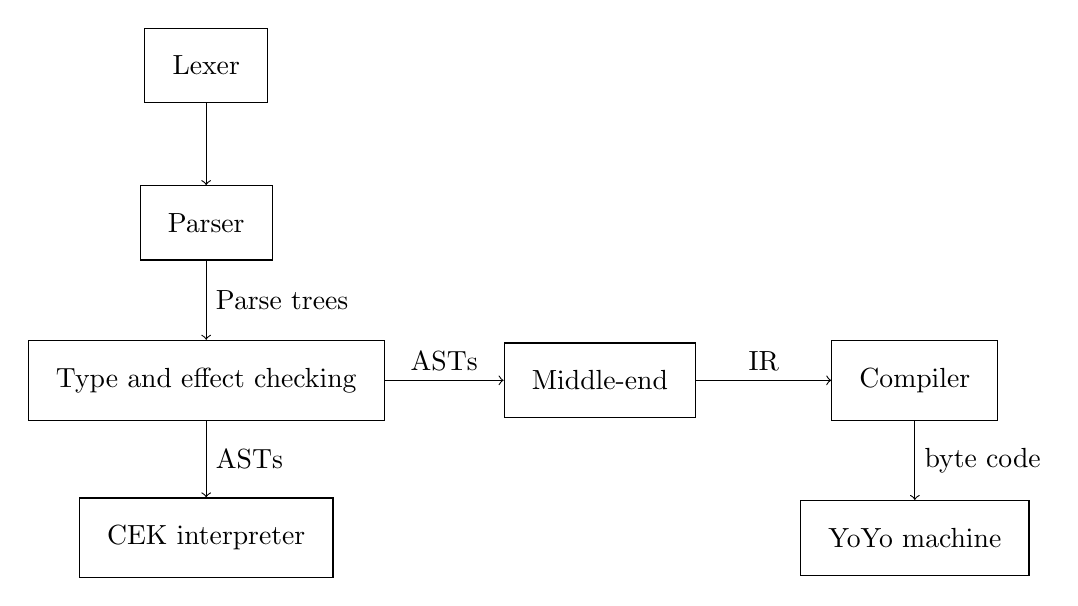
\begin{tikzpicture}
    \node[draw,inner sep=10pt] (LEX) at (0,6) {Lexer};
    \node[draw,inner sep=10pt] (PAR) at (0,4) {Parser};
    \node[draw,inner sep=10pt] (TYPE) at (0,2) {Type and effect checking};
    \node[draw,inner sep=10pt] (MID) at (5, 2) {Middle-end};
    \node[draw,inner sep=10pt] (COMP) at (9,2) {Compiler};
    \node[draw,inner sep=10pt] (CEK) at (0,0) {CEK interpreter};
    \node[draw,inner sep=10pt] (YOYO) at (9,0) {YoYo machine};
    
    \draw[->] (LEX) -- (PAR);
    \draw[->] (PAR) -- (TYPE) node[midway, right] {Parse trees};
    \draw[->] (TYPE) -- (CEK) node[midway, right] {ASTs};
    \draw[->] (TYPE) -- (MID) node[midway, above] {ASTs};
    \draw[->] (MID) -- (COMP) node[midway, above] {IR};
    \draw[->] (COMP) -- (YOYO) node[midway, right] {byte code};
  \end{tikzpicture}}
  \caption{Structure of the project}
  \label{fig:project-structure}
\end{figure}

\section{Summary}
This section summed up the theory background which was needed to complete this dissertation.
It also shows the preparation I undertook in the software engineering aspects of the project.

\begin{itemize}
  \item I briefly introduced the programming language Eff and talked about its characteristic features. I showed
    code examples demonstrating how handlers can be used.
  \item I explained the idea of a continuation, how it represents an arbitrary program point in the
    execution of a program and how it allows advanced control flow to be implemented.
  \item I gave an overview of control operators (including Landin's J operator), why they were studied in the 
    early days of programming languages and their rôle in the development of different virtual machines.
  \item I talked about the small-step operational semantics of core Eff as well as the typing of Eff terms.
  \item I mentioned two abstract machines which can implement the structured \emph{non-local
    flow of control} continuations make possible. The key challenge these machines solve is that
    they can \emph{save and restore} execution contexts in an appropriate way whenever non-local control flow occurs.

    A CEK machine does this by keeping a stack of continuations (K), while the SECD machine does this by using
    a so-called dump (D). The importance of these machines will become clearer in the Implementation section where I describe the
    Yoyo virtual machine for Eff which has similarities with both of these abstract machines.
  \item I stated my starting point, the timeline of my project and discussed the development methodology used
    to write the code and the testing strategy to assess its correctness.
\end{itemize}


\begin{comment}
\subsection{Eff}

This subsection gives a short introduction to Eff with some code examples.
The precise syntax and semantics of the language will be defined later,
we aim for an intuitive introduction here.

\subsubsection{Effects}

There is an important distinction between syntactic and semantic elements in the language. Effect declarations belong to syntax.

An effect in Eff is declared using the \verb|effect| keyword together with a type signature which forms the effect signature. One would define a \verb|Print| effect for printing strings as follows:



This tells us two things. To invoke the \verb|Print| effect we must provide a string as an argument and what we get back is something of type \verb|unit| after the effect is performed. We get to know no extra information about \verb|Print|.

Now that we have a \verb|Print| effect we can write down the mandatory Hello World example:
\begin{verbatim}
perform (Print "Hello World!")
\end{verbatim}

The \verb|perform| keyword is used to perform already declared effects. However, if we think about it, this piece of code still does
not make any sense as we don't know how to interpret \verb|Print "Hello World!"|.

\subsubsection{Handlers}

Handlers are used to assign meaning to effects. A handler is just a list of rules. A rule can be of three different types: a value rule, an effect rule or a finally rule.

\textbf{Value and effect rules}

The following handler provides an interpretation for the \verb|Print| effect. This handler converts the result of a computation to a 2-tuple where the first element is the original result and the second
element is a concatenation of the strings from all the \verb|Print| effects from the computation.

We use the value rule \verb|v -> (v, "")| to say what happens ``by default''. If the computation didn't print anything then we simply say that it printed the empty string.

\begin{verbatim}
let collect = handler
| v -> (v, "")
| effect (Print str) k ->
    (* Find out what the rest of the computation would print out *)
    let (result, s) = continue k () in
    (* Prefix the string printed by the rest of the computation 
       with `str` from this effect *)
    (result, str ^ s)
\end{verbatim}

The effect rule is a bit more involved. Effect rules have the form \verb|effect E(args) k| where \verb|k| is always bound to the ``rest of the computation'' which we call a continuation (and by convention
usually use the letter $k$ or $\kappa$ to denote it). The arguments of the effect \verb|E| are bound to \verb|args| via pattern matching. In the example above we first resume the computation by resuming the
computation via \verb|continue|. After we find out what the rest of the computation would print out, we prepend our current string to it.

Note that when we handle an effect of type $\alpha \to \beta$ we get a continuation of type $\beta \to \gamma$ where $\gamma$ is the type of the computation being enclosed in a \verb|with ... handle| block.

Value rules can be omitted in handler definitions, in which case they are assumed to be identities.

\textbf{Finally rules}

Finally rules are just syntactic sugar for \verb|let| wrappers around \verb|with ... handle| statements that act on the result of a handled computation, i.e.,
\begin{verbatim}
let h = handler
    | finally x -> x + x
in 
    with h handle c
\end{verbatim}
would be syntactic sugar for
\begin{verbatim}
let x = with h handle c in x + x.
\end{verbatim}

I would like to point out that this syntax is added only for convenience as it happens many times that the same transformations must be performed after a \verb|with ... handle| block \cite{bauer2015programming}. Hence \verb|finally| here does not provide the Java-like semantics where the computation in a finally block is ``guaranteed'' to be executed.

Finally rules can be omitted in handler definitions, in which case they are assumed to be identities.

\textbf{Handler types}

Handlers handling a computation of type $\alpha$ and giving a result of type $\beta$ are given the type $\alpha \Rightarrow \beta$.
\end{comment}

\begin{comment}
\subsection{TODOs}
\begin{itemize}
\item I haven't said anything about shallow and deep handlers
\item Comparing to haskell monads/monad transformers is risky -- need to explain these
\end{itemize}

\section{Papers}
\begin{itemize}
\item Delimited control \cite{kiselyov2010delimited}
\item Eff Directly in OCaml \cite{Kiselyov_2018}
\item Very good article about CPS compilation \cite{flanagan1993essence}
\item Bauer tutorial \cite{bauer2018algebraic}
\end{itemize}
\end{comment}

\ifstandalone
\bibliography{../bibliography}{}
\bibliographystyle{plain}
\fi

\end{document}